
% ---------- Titelblad Masterproef Faculteit Wetenschappen -----------
% Dit document is opgesteld voor compilatie met pdflatex. Indien je
% wilt compileren met latex naar dvi/ps, dien je de figuren naar
% (e)ps-formaat om te zetten.
% -- december 2012
% -------------------------------------------------------------------
\RequirePackage{fix-cm}
\documentclass[12pt,a4paper,oneside]{article}
% --------------------- In te laden pakketten -----------------------
% Deze kan je eventueel toevoegen aan de pakketten die je al inlaadt
% als je dit titelblad integreert met de rest van thesis.
% -------------------------------------------------------------------
\usepackage{graphicx,textpos}
\usepackage[usenames,dvipsnames]{xcolor}
\usepackage{helvet}
% -------------------- Pagina-instellingen --------------------------
% Indien je deze wijzigt, zal het titelblad ook wijzigen. Dit dien je
% dan manueel aan te passen.
% --------------------------------------------------------------------
\topmargin -10mm
\textwidth 160truemm
\textheight 240truemm
\oddsidemargin 0mm
\evensidemargin 0mm
% ------------------- textpos-instellingen ---------------------------
% Enkele andere instellingen voor het voorblad.
% --------------------------------------------------------------------
\definecolor{green}{RGB}{172,196,0}
\definecolor{bluetitle}{RGB}{29,141,176}
\definecolor{blueaff}{RGB}{0,0,128}
\definecolor{blueline}{RGB}{82,189,236}
\setlength{\TPHorizModule}{1mm}
\setlength{\TPVertModule}{1mm}
%----------------------- Custom stuff -------------------------------
\graphicspath{./}
\usepackage{makeidx}
\index{hoofd}
\makeindex
\usepackage{amsmath}
\usepackage[english]{babel}
\usepackage{hyperref}
%------------------------ Plot packages ----------------------------
\usepackage{tikz}
\usepackage{standalone}
\usepackage{pgfplots}
\usepackage{pgf}
\usepackage{units}
\usepackage{metalogo}
\usepackage{graphicx}
\usepackage{caption}
\usepackage{subcaption}
%------------------------ Lisings ----------------------------------
\usepackage{listings} 


%\lstset{emph={trueIndex,root},emphstyle=\color{BlueViolet}}%\underbar} % for special keywords
\lstset{language=[LaTeX]Tex,%C++,
    keywordstyle=\color{blue},%\bfseries,
    basicstyle=\small\ttfamily,
    %identifierstyle=\color{NavyBlue},
    commentstyle=\color{Green}\ttfamily,
    stringstyle=\rmfamily,
    numbers=none,%left,%
    numberstyle=\scriptsize,%\tiny
    stepnumber=5,
    numbersep=8pt,
    showstringspaces=false,
    breaklines=true,
    frameround=ftff,
    frame=single,
    belowcaptionskip=.75\baselineskip
    %frame=L
} 
%----------------------Title etc----------------------------------
\title{NUMERICAL SIMULATION OF PARTIAL DIFFERENTIAL EUQATIONS IN TWO DIMENSIONS.}
\author{Vincent Peeters $ \& $ Moritz Wolter}
\date{\today}
% --------------------------------------------------------------------


\begin{document}
\maketitle

\section{Implementation of explicit methods}
In this report we are going to implement explicit methods to solve three different partial differential equations in two dimensions and analyze the results.
\subsection{Heat Equation}
We will begin with the numerical solution of the heat equation:
\begin{equation}
\frac{\partial u}{\partial t} = \frac{\partial^2 u}{\partial x^2} + \frac{\partial^2 u}{\partial y^2}.
\end{equation}
From the lecture we know that this problem may be solved by extension of the one dimensional explicit scheme:
\begin{equation}
\frac{U^{n+1}-U^{n}}{\triangle t} = b [\frac{\delta_x^2 U^n}{(\triangle x)^2} + \frac{\delta_y^2 U^n}{(\triangle y)^2} ].
\end{equation}
with b = 1 in our case. By expanding the central differences we arrive at:
\begin{equation}
U_{r,x}^{n+1} = U_{r,s}^n (1 - 2\mu_x - 2\mu_y) + \mu_x U_{r+1,s}^n + \mu_x U_{r-1,s}^n + \mu_y U_{r,s+1}^n + \mu_y U_{r,s-1}^n.
\label{eq:heat}
\end{equation}
Equation~\ref{eq:heat} my be implemented in matlab. With $\mu_x = \frac{\triangle t}{(\triangle x)^2}$ and $\mu_y = \frac{\triangle t}{(\triangle y)^2}$. As we are using a symmetric grid we have $\mu_x = \mu_y$ which leads to the implementation in listing~\ref{lst:expHeat}: 
\lstinputlisting[language=matlab,caption={Explicit solution of the heat equation in two dimensions.},label=lst:expHeat,captionpos=b]{code/heat2d.tex}

\subsection{Wave equation}
Next we are going to implement an explicit scheme to solve the wave equation:
\begin{equation}
\frac{\partial^2 u}{\partial t^2} = \frac{\partial^2 u}{\partial x^2} + \frac{\partial^2 u}{\partial y^2}.
\end{equation}
Approximating the second derivatives with central differences and solving for $U_{r,s}^{n+1}$ we obtain the scheme:
\begin{align*}
U_{r,s}^{n+1} = U_{r,s}(2 - 2\mu_x - 2 \mu_y) - U_{r,s}^{n-1} \\
				 + \mu_x U_{r-1,s}^n + \mu_x U_{r+1,s}^n	  \\
				 + \mu_y U_{r,s-1}^n + \mu_y U_{r,s+1}.
\end{align*}
With $\mu_x = \frac{(\triangle t)^2}{(\triangle x)^2} $ and $\mu_y = \frac{(\triangle t)^2}{(\triangle y)^2} $. In comparison to listing~\ref{lst:expHeat} when listing only changes to the for loop. We got:
\lstinputlisting[language=matlab,caption={Code for solving the wave equation.},label=lst:expWave,captionpos=b]{code/waveFor.tex}
Obviously different initial parameters will have to be chosen here.


\subsection{Transport equation}
Before we are going to consider the numerical stability and accuracy of these methods we will implement a final scheme to solve the transport equation:
\begin{equation}
\frac{\partial u}{\partial t} = \frac{\partial u}{\partial x} + \frac{\partial u}{\partial y}.
\end{equation} 
Using exclusively forward differences to approximate the first order differentials and solving for $U_{r,s}^{n+1}$ once more we obtain:
\begin{equation}
U_{r,s}^{n+1} = U_{r,s}^n (1 - \mu_x - \mu_y) + \mu_x U_{r+1,s} + \mu_y U_{r,s+1}.
\end{equation}
With $\mu_x = \frac{\triangle t}{\triangle x} $ and $\mu_y = \frac{\triangle t}{\triangle y} $ .Which leads to the modified for-loop for the transport case:
\lstinputlisting[language=matlab,caption={Code for solving the two dimesional transport equation.},label=lst:expWave,captionpos=b]{code/transportFor.tex}


\section{Analysis}
\subsection{Stability}
Figure~\ref{fig:stableUnstable} shows stable and unstable solutions for the three equations. We will proceed with taking a close look at the numerical properties of the methods we described so far. 
\begin{figure}
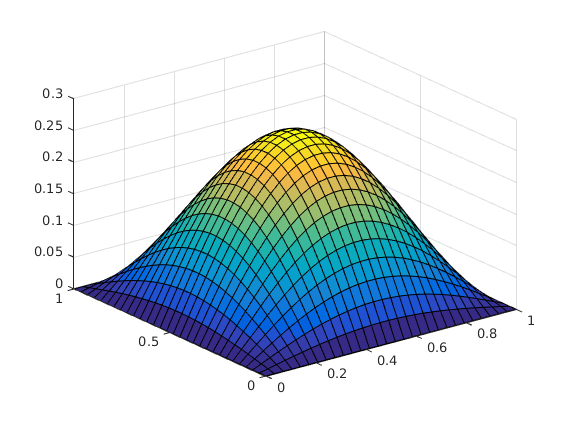
\includegraphics[scale = 0.33]{images/heat.png}
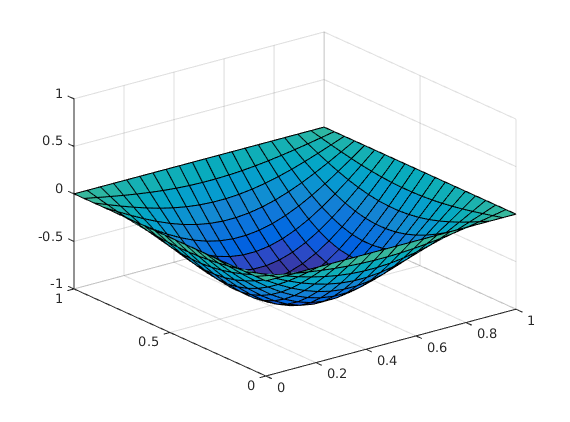
\includegraphics[scale = 0.33]{images/wave.png}
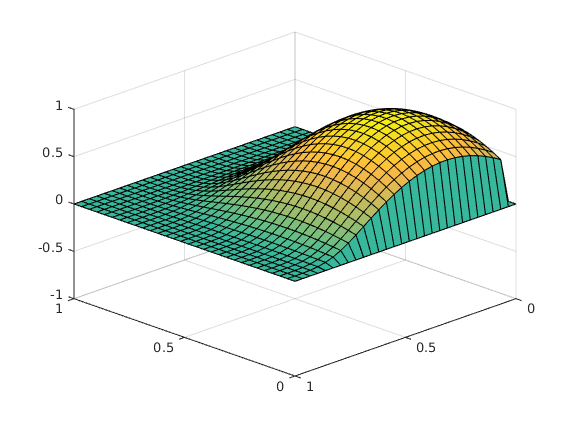
\includegraphics[scale = 0.33]{images/transport.png}
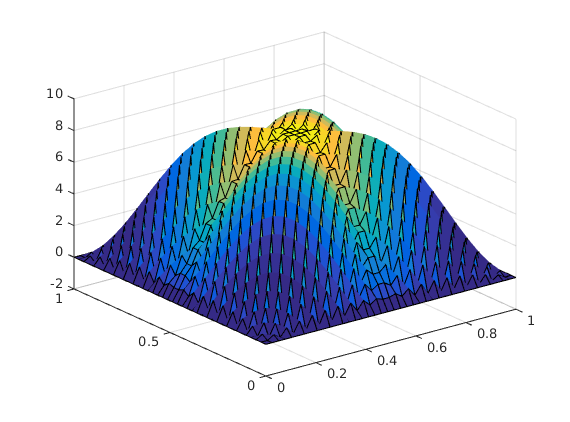
\includegraphics[scale = 0.33]{images/heatUnstable.png}
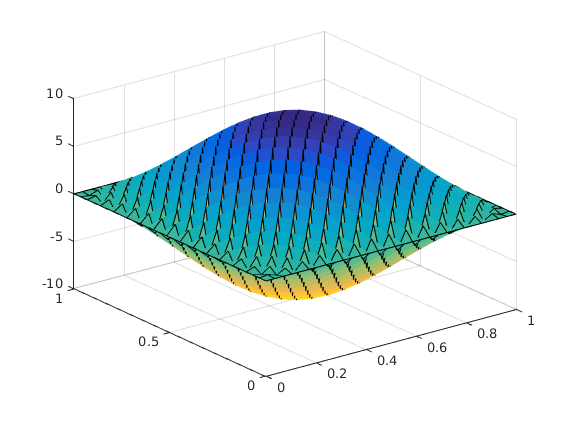
\includegraphics[scale = 0.33]{images/waveUnstable.png}
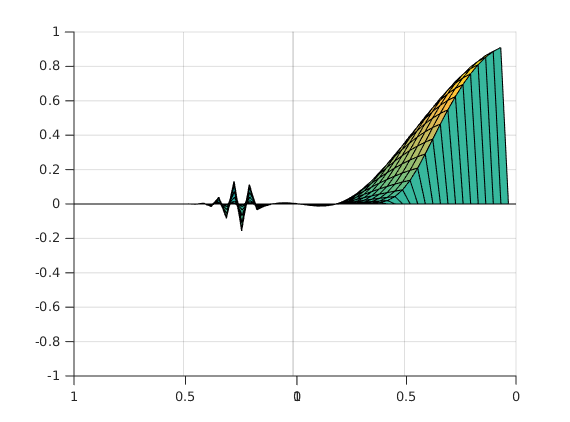
\includegraphics[scale = 0.33]{images/transportUnstable.png}
\caption{Numerical solutions computed using the schemes described above for stable (top row) and unstable (bottom row) grid ratios $\mu$.}
\label{fig:stableUnstable}
\end{figure}
In order to obtain stable solutions in two dimensions we have to satisfy the condition:
\begin{equation}
\mu_x + \mu_y \leq 0.5
\end{equation}
For equally spaced with $\mu_x = \mu_y = \mu$ grids we get:
\begin{equation}
\mu \leq 0.25
\end{equation}
Where $\mu_x$ and $\mu_y$ are different for every method, as derived in the previous section. For the following computations we kept $J=30$, defined $\triangle x = \triangle y = 1/J$ and computed $dt$ from mu. For the heat equation for the solution in figure~\ref{fig:stableUnstable} in the top left is stable here we have $\mu = 0.25 = \mu_x = \mu_y$ at $t=1$. However to compute the image in the bottom left we used a grid ratio of $\mu = 0.252$ and we observe instability at the same point in time. The solution of the wave equation is shown in the top middle position for time t=1 with $\mu = 0.25$. We found the wave equation to be surprisingly stable. In our computations first instabilities appeared at time $t = 10$ with a grid ratio of $\mu = 0.51$. The transport problem also turned out to be more stable then the heat equation. In the top right corner of figure~\ref{fig:stableUnstable} we show the solution of the transport equation for the given initial condition at time $0.5$. First instabilities at this time appeared with a grid ratio of $\mu = 0.6$, which are shown below.



\subsection{Accuracy}
\subsubsection{Exact Solution of the Heat Equation}
By using the ansatz $u = T(t)Y(y)X(x)$ followed by separation of variables and using the initial conditions we arrived at the exact solution:
\begin{equation}
U(x,y,t) = e^{-2\pi^2 t}sin(\pi x)sin(\pi y).
\end{equation}
Which indeed satisfies the differential equation.
\subsubsection{Exact Solution of the Wave Equation}
Again using the same Idea we propose the solution:
\begin{equation}
u(x,y,t) = cos(\sqrt{2}\pi t)sin(\pi x)sin(\pi y).
\end{equation}
which indeed satisfies the partial differential equation.
\subsubsection{Exact Solution of Transport Equation}
As a solution for the transport equation of form

\begin{equation}
\frac{\delta u}{\delta t} = \frac{\delta u}{\delta x} + \frac{\delta u}{\delta y}
\end{equation}
with a given initial conditions, $u_0(x,y)$, and homogenous dirichet boundary conditions we propose a solution of the following form:
\begin{equation}
u(x,y,t) = u_0(x-vt,y-vt)
\label{proposal}
\end{equation}
Calculating the partial derivatives found in the transport equation we get
\begin{equation}
\frac{\delta u}{\delta t} =(-v) \frac{\delta u_0(x,y)}{\delta x} +(-v) \frac{\delta u_0(x,y)}{\delta y} 
\end{equation}

\begin{equation}
\frac{\delta u}{\delta x} = \frac{\delta u_0(x,y)}{\delta x} ,\frac{\delta u}{\delta y} = \frac{\delta u_0(x,y)}{\delta y} 
\end{equation}
Filling this then in the transport equation gives

\begin{equation}
-v\frac{\delta u_0}{\delta x}-v\frac{\delta u_0}{\delta y} = \frac{\delta u_0}{\delta x}+\frac{\delta u_0}{\delta y} 
\end{equation}

which fits when $v=-1$ and so our solution is
\begin{equation}
u(x,y,t)=u_0(x+t,y+t)
\end{equation}

\subsection{Error analysis of our scheme for the heat equation}
TODO...
\subsection{Error analysis of our scheme the wave equation}
TODO...


\subsubsection{Error analysis of the transport problem}

The truncation error for the upwind scheme with $a=1$ can be found to be

\begin{equation}
T_j^n = -\frac{1}{2}(1-\nu)\Delta x u_{xx} + ...
\end{equation}
Which is first order in $\Delta x$, and therefore, under constant $\nu$, also first order in $\Delta t$.

We then now that the maximum error $E^n$ at a point in time $n$ is bound by a function of the same order. And this is what we see in figure \ref{errororrrTransport}

\begin{figure}[htbp] %  figure placement: here, top, bottom, or page
   \centering
   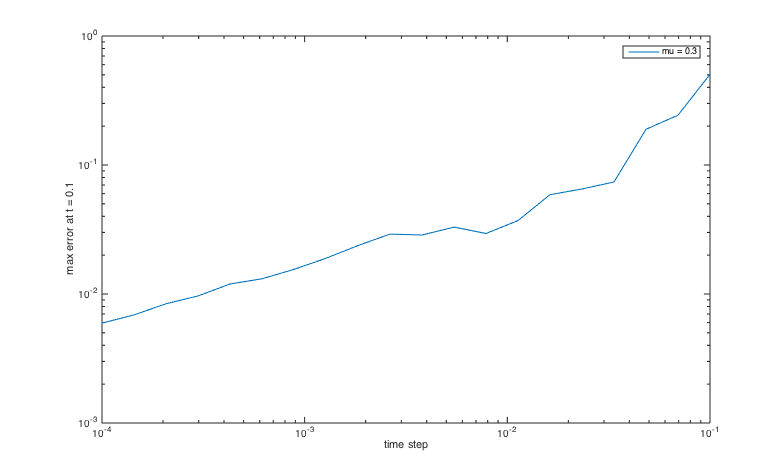
\includegraphics[scale=0.3]{images/errororrrTransport} 
   \caption{The maximum error at time = 0.1 in function of the tilmestep at a constant $\nu$ of 0.3 }
   \label{errororrrTransport}
\end{figure}




\section{Another initial solution}
Finally we are going to compute the solutions again with the initial solution:
\begin{equation}
u_0(x,y) = 15(x-x^2)(y - y^2) e^{-50(x-0.5)^2 + (y-0.5)^2}
\end{equation}
Figure~\ref*{fig:part4} shows the results.\footnote{For solution of the wave equation, which we found exepctionally pretty a video may be downloaded from: \url{https://www.youtube.com/watch?v=gE13nlbE5ug&feature=youtu.be}}. It is important to note that the solution of the heat equation disappears extremely quickly. The maximum is of scale $10^{-2}$ at time $t = 0.1$ and decreases to $10^{-3}$ at $t=0.2$.

\begin{figure}
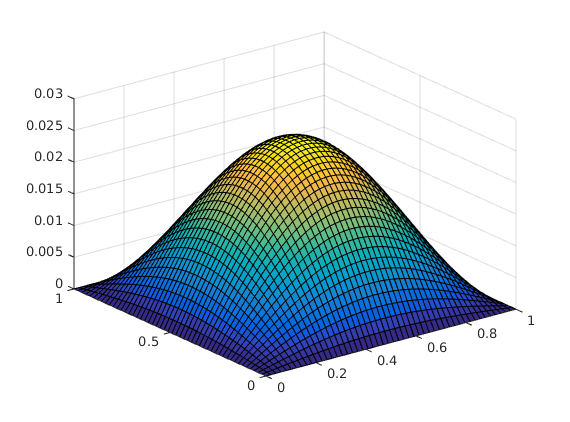
\includegraphics[scale=0.33]{images/heatP4T01.png}
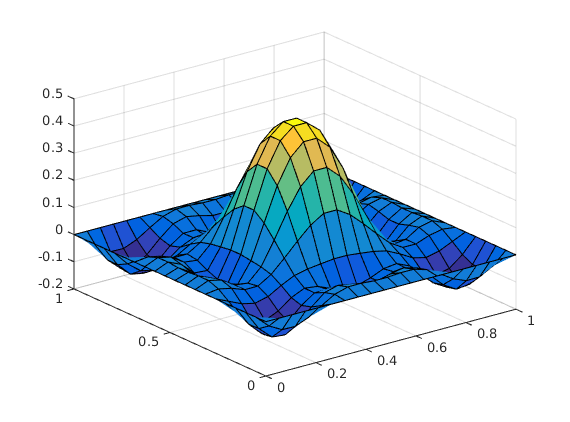
\includegraphics[scale=0.33]{images/waveP4T01.png}
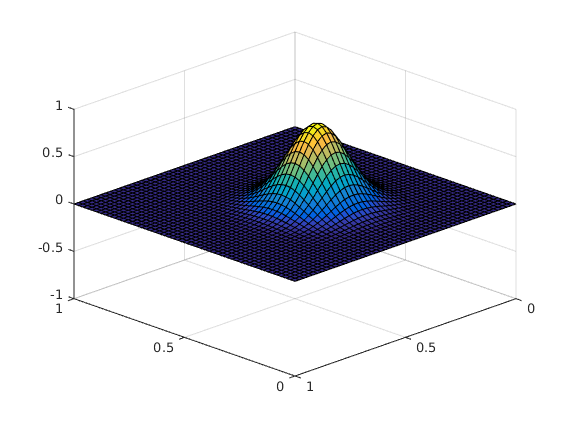
\includegraphics[scale=0.33]{images/transpP4T01.png}
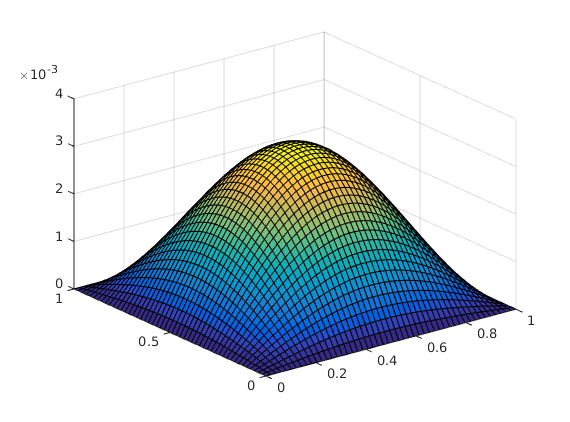
\includegraphics[scale=0.33]{images/heatP4T02.png}
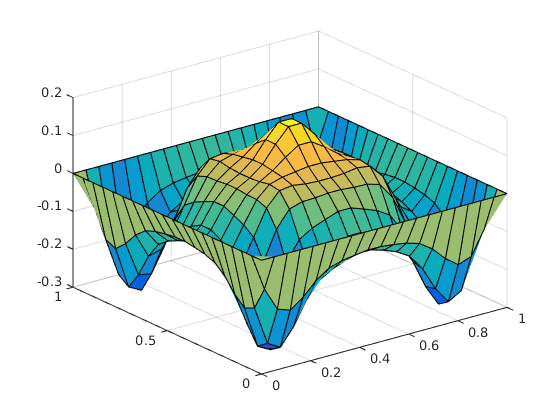
\includegraphics[scale=0.33]{images/waveP4T02.png}
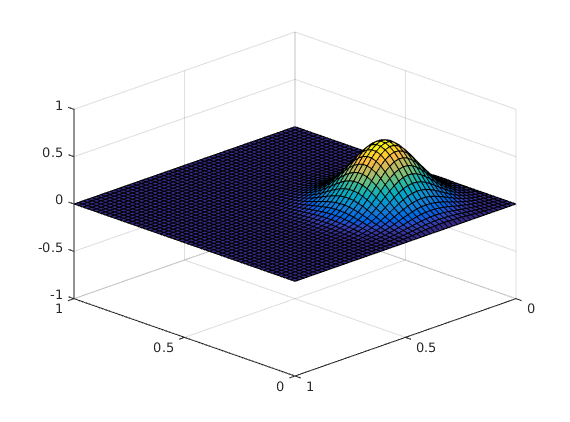
\includegraphics[scale=0.33]{images/transpP4T02.png}
\caption{The tree equations with $\mu_x=\mu_y= 0.1$ at $t = 0.1$ (top row) and $t = 0.2$ (bottom row). }
\label{fig:part4}
\end{figure}

\end{document}
